\addcontentsline{toc}{section}{Appendix} % Remove this if you don't want the appendix included in the table of contents.
\appendix

\section{Plots}\label{sec:plots}

\begin{figure}[h]
	\centering
	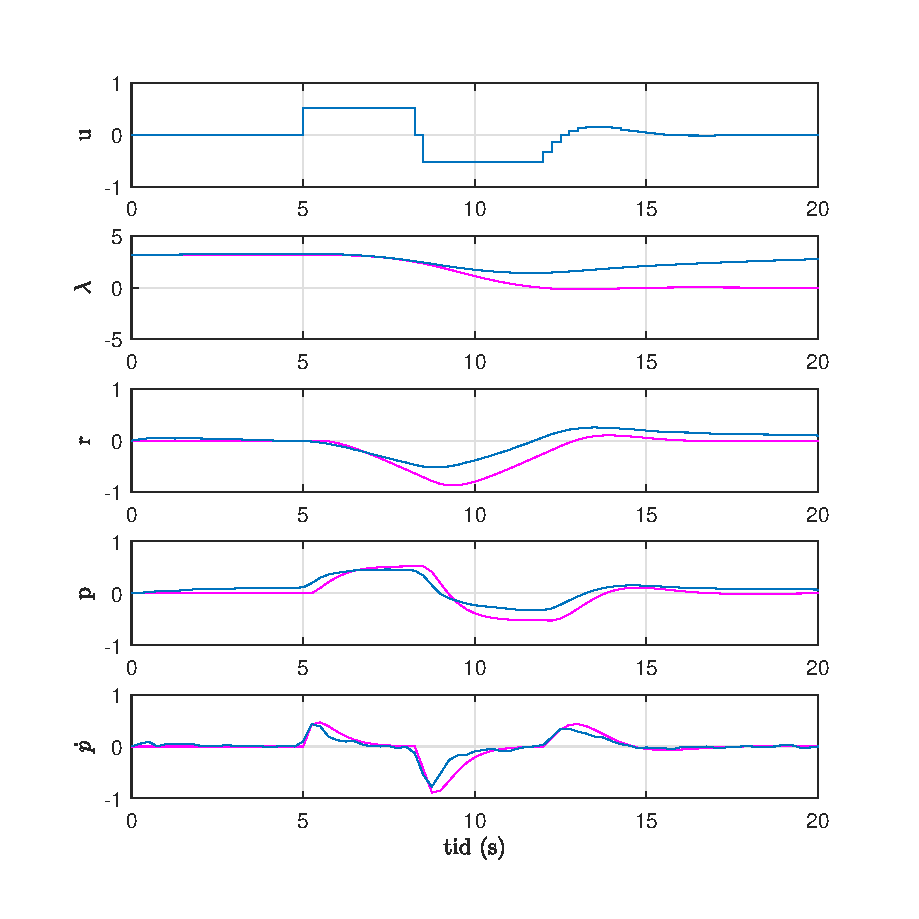
\includegraphics[width=\textwidth]{figures/plots/2_P1=01.eps}
	\caption{Optimal trajectory in magenta and measured states in blue, no feedback and $P_1=0.1$.}
\label{fig:2_p1=0.1}
\end{figure}

\begin{figure}[h]
	\centering
	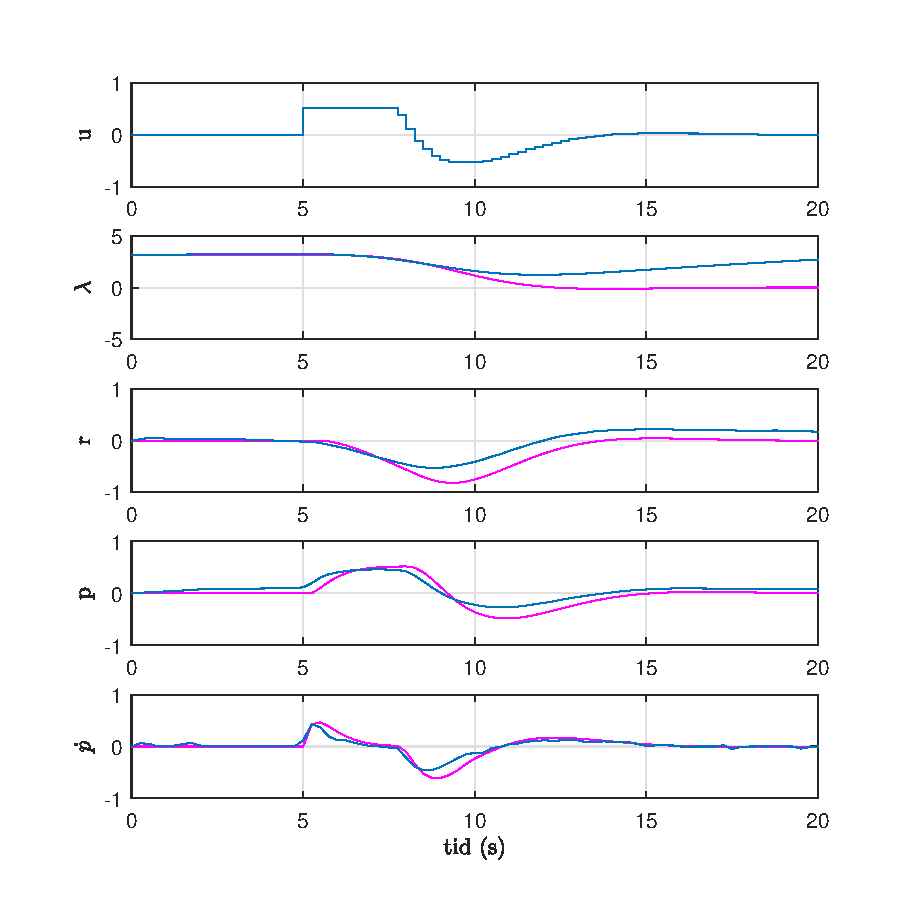
\includegraphics[width=\textwidth]{figures/plots/2_P1=1.eps}
	\caption{Optimal trajectory in magenta and measured states in blue, no feedback and $P_1=1$.}
\label{fig:2_p1=1}
\end{figure}

\begin{figure}[h]
	\centering
	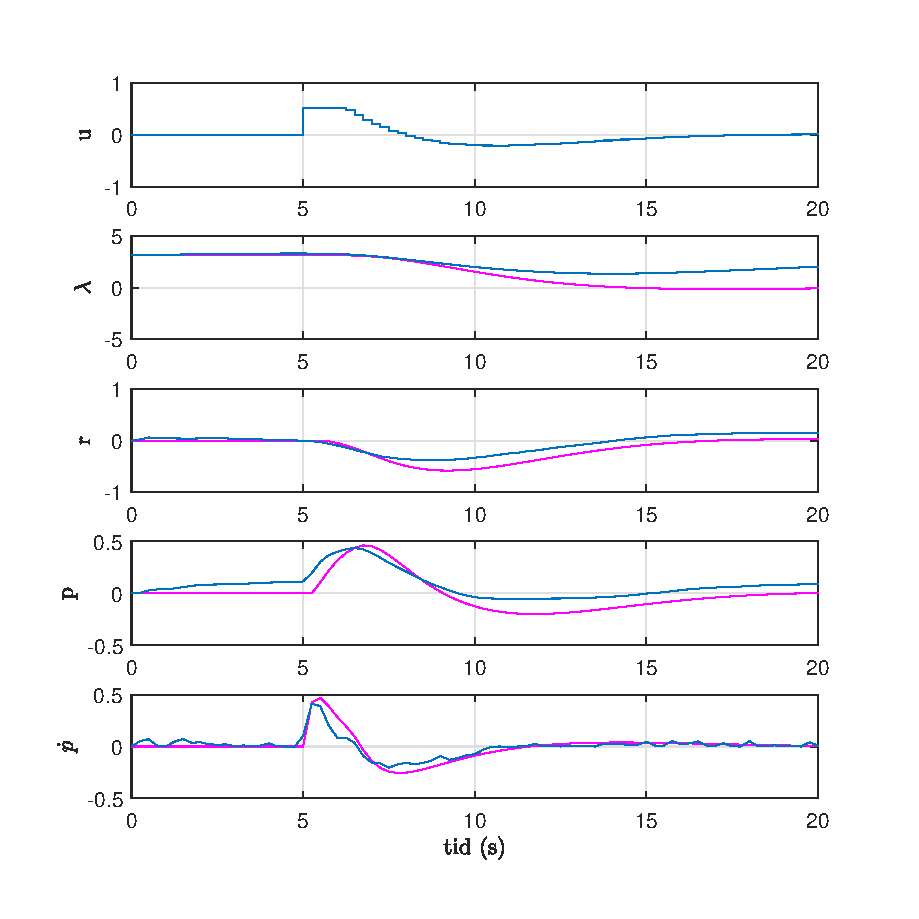
\includegraphics[width=\textwidth]{figures/plots/2_P1=10.eps}
	\caption{Optimal trajectory in magenta and measured states in blue, no feedback and $P_1=10$.}
\label{fig:2_p1=10}
\end{figure}

\begin{figure}[h]
	\centering
	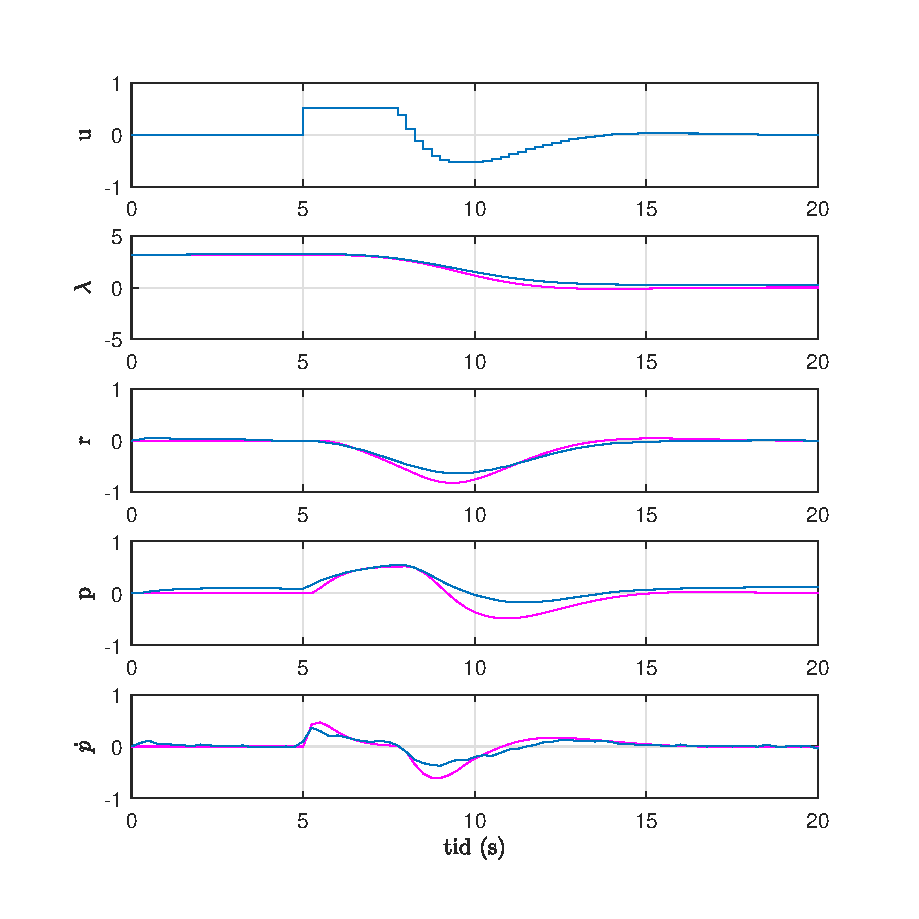
\includegraphics[width=\textwidth]{figures/plots/3_R=01.eps}
	\caption{Optimal trajectory in magenta and measured states in blue, with feedback and $P_1=1$ and $R=0.1$.}
\label{fig:3_r=0.1}
\end{figure}

\begin{figure}[h]
	\centering
	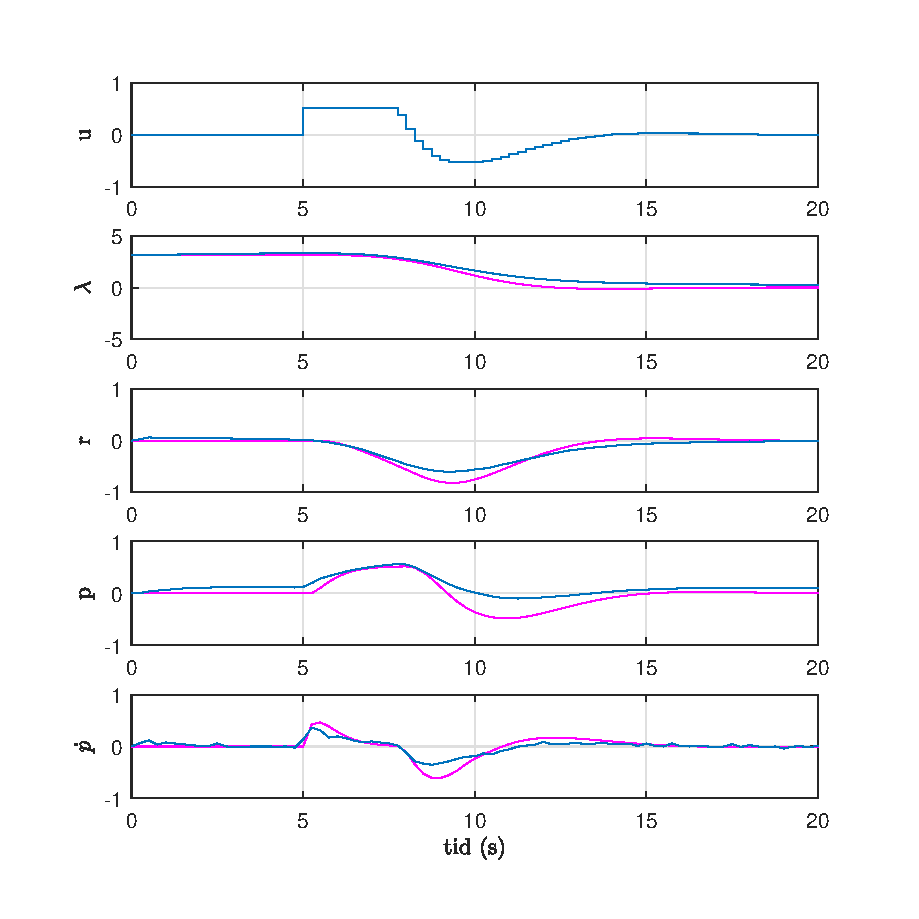
\includegraphics[width=\textwidth]{figures/plots/3_R=1.eps}
	\caption{Optimal trajectory in magenta and measured states in blue, with feedback and $P_1=1$ and $R=1$.}
\label{fig:3_r=1}
\end{figure}

\begin{figure}[h]
	\centering
	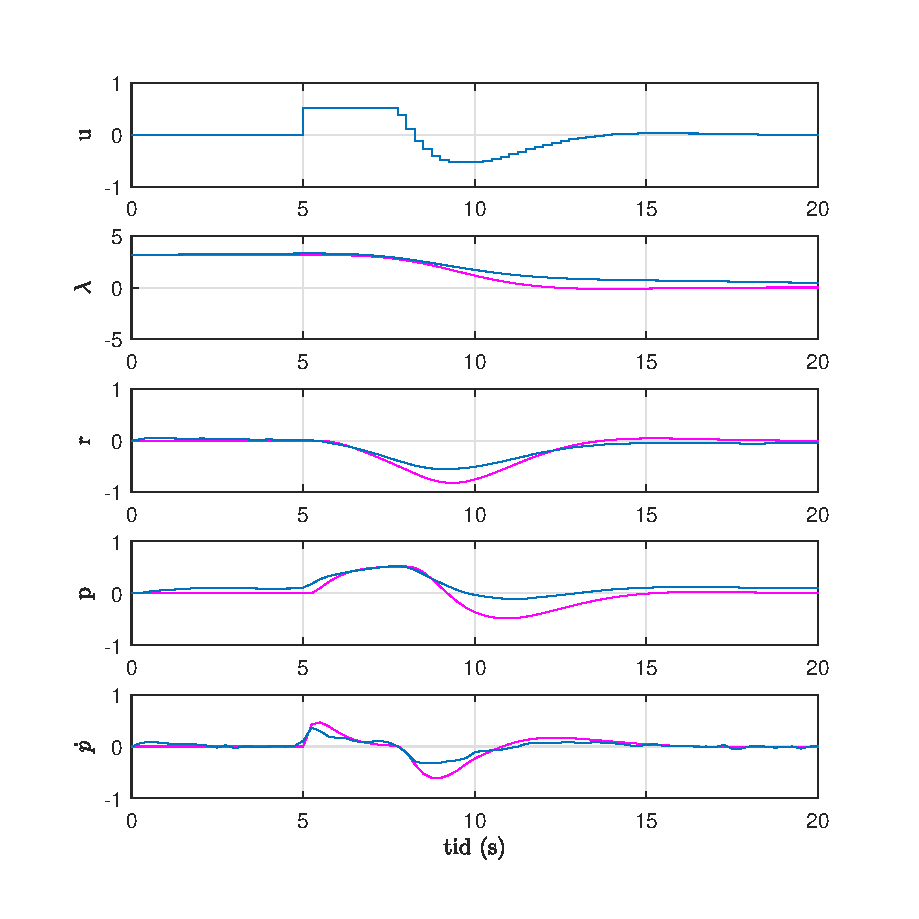
\includegraphics[width=\textwidth]{figures/plots/3_R=10.eps}
	\caption{Optimal trajectory in magenta and measured states in blue, with feedback and $P_1=1$ and $R=10$.}
\label{fig:3_r=10}
\end{figure}

\begin{figure}[h]
	\centering
	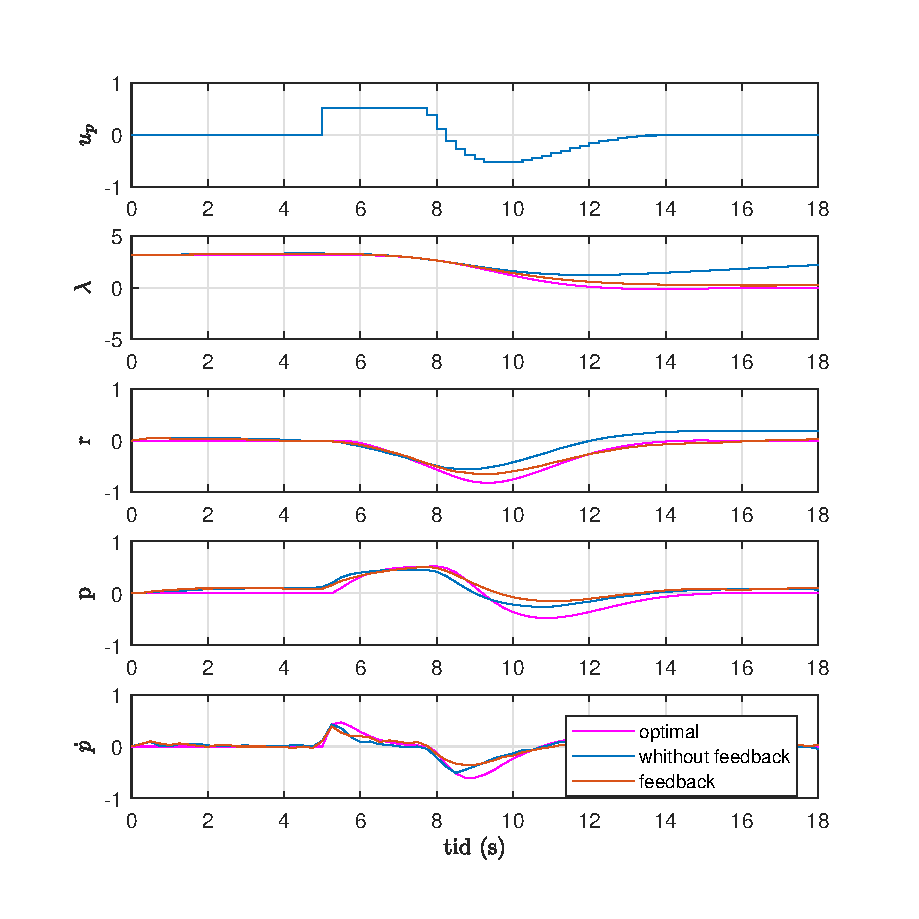
\includegraphics[width=\textwidth]{figures/plots/4_fb_vs_no_fb_UNTUNED_pitch_legend.eps}
	\caption{Comparison of feedback and no feedback for the extended system with untuned parameters. Showing the pitch-dependent states.}
\label{fig:4_untuned_pitch}
\end{figure}

\begin{figure}[h]
	\centering
	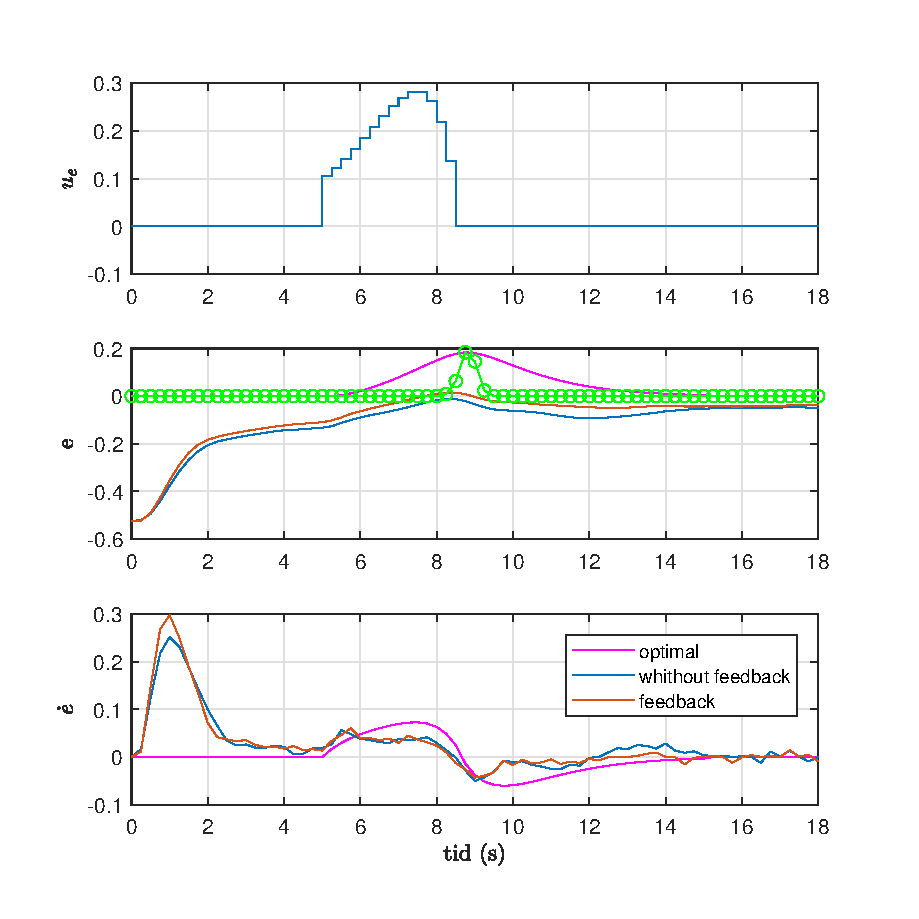
\includegraphics[width=\textwidth]{figures/plots/4_fb_vs_no_fb_UNTUNED_elev.eps}
	\caption{Comparison of feedback and no feedback for the extended system with untuned parameters. Showing the elevation-dependent states. Obstacle plotted in green.}
\label{fig:4_untuned_elev}
\end{figure}

\begin{figure}[h]
	\centering
	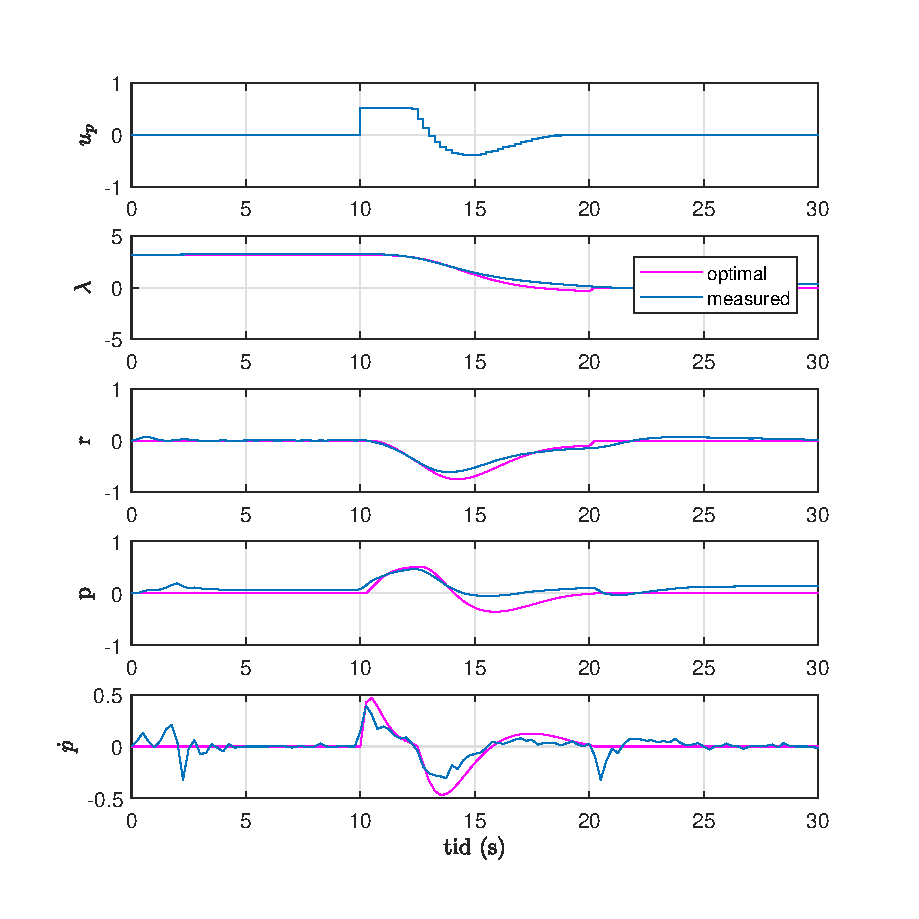
\includegraphics[width=\textwidth]{figures/plots/4_tuned_legend_pitch.eps}
	\caption{Tuned response of the helicopter compared to the optimal trajectory. Showing pitch-dependant states.}
\label{fig:4_tuned_pitch}
\end{figure}

\begin{figure}[h]
	\centering
	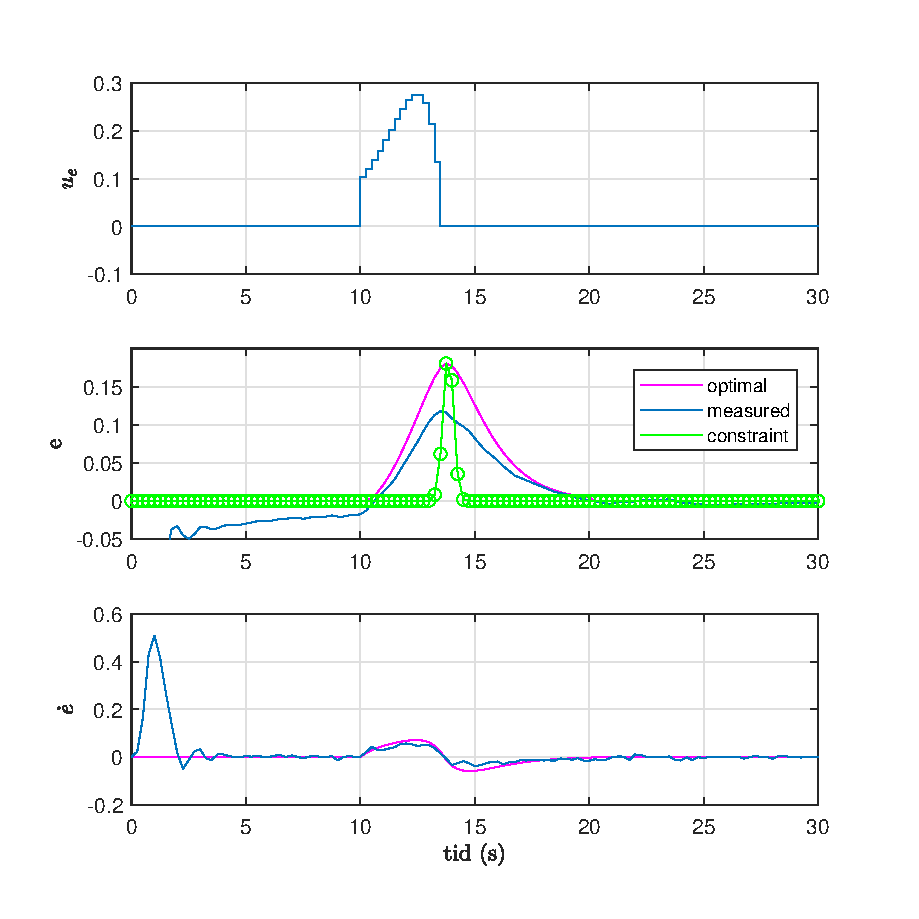
\includegraphics[width=\textwidth]{figures/plots/4_tuned_elev.eps}
	\caption{Tuned response of the helicopter compared to the optimal trajectory. Showing elevation-dependant states. Obstacle plotted in green.}
\label{fig:4_tuned_elev}
\end{figure}

\begin{figure}[h]
	\centering
	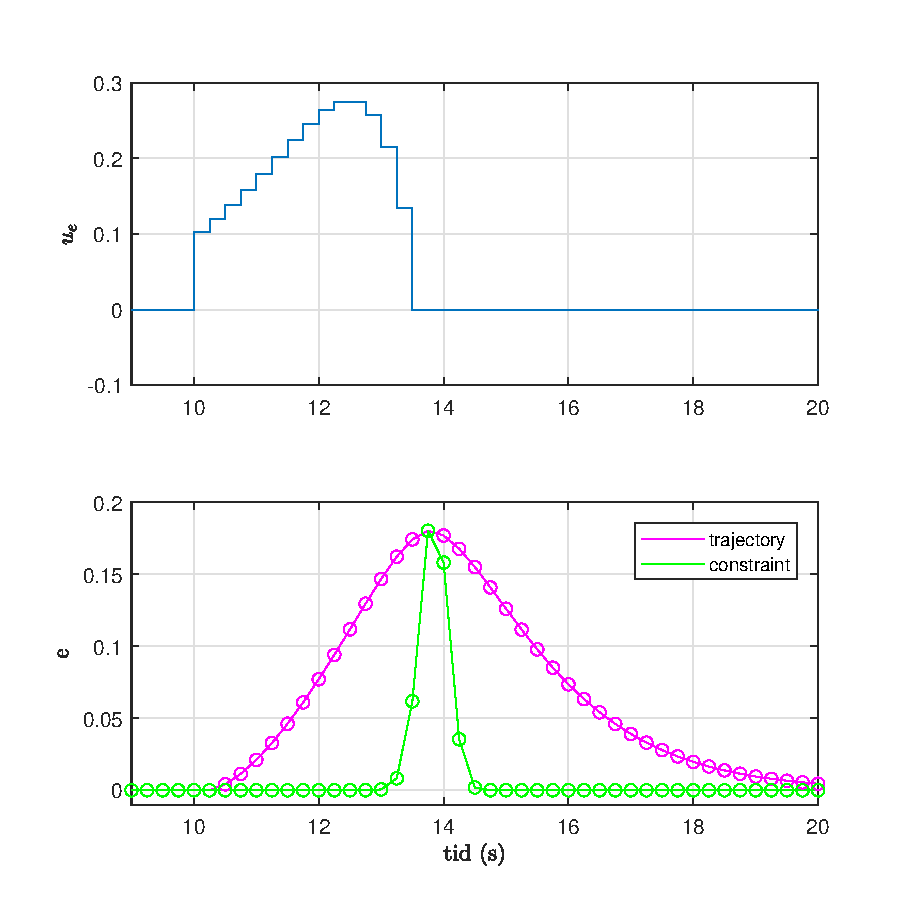
\includegraphics[width=\textwidth]{figures/plots/4_opt_trajectory_over_hill.eps}
	\caption{Plot of optimal trajectory over the obstacle constraint.}
\label{fig:4_hill_trajec}
\end{figure}

\clearpage
\section{MATLAB Code}\label{sec:code}

\sloppy
\definecolor{lightgray}{gray}{0.5}
\setlength{\parindent}{0pt}

    
\subsection{init.m}\label{sec:init}
\begin{verbatim}
clear all;
close all;
clc;

%Physical constants
m_h = 0.4; % Total mass of the motors.
m_g = 0.03; % Effective mass of the helicopter.
l_a = 0.65; % Distance from elevation axis to helicopter body
l_h = 0.17; % Distance from pitch axis to motor

% Moments of inertia
J_e = 2 * m_h * l_a *l_a;         % Moment of interia for elevation
J_p = 2 * ( m_h/2 * l_h * l_h);   % Moment of interia for pitch
J_t = 2 * m_h * l_a *l_a;         % Moment of interia for travel

% Identified voltage sum and difference
V_s_eq = 4.7; % Identified equilibrium voltage sum.
V_d_eq = 0.0; % Identified equilibrium voltage difference.

% Model parameters
K_p = m_g*9.81; % Force to lift the helicopter from the ground.
K_f = K_p/V_s_eq; % Force motor constant.
K_1 = l_h*K_f/J_p;
K_2 = K_p*l_a/J_t;
K_3 = K_f*l_a/J_e;
K_4 = K_p*l_a/J_e;
\end{verbatim}

\subsection{problem\_2.m}\label{sec:p2}
\begin{verbatim}
%Initialization and model definition

clc;
clear;

init; % Change this to the init file corresponding to your helicopter

% Discrete time system model. x = [lambda r p p_dot]'
delta_t	= 0.25; % sampling time
A1 = [1   delta_t       0                  0;
      0     1    -delta_t*K_2              0;
      0     0           1               delta_t;
      0     0  -delta_t*K_1*K_pp   1 - delta_t*K_1*K_pd];
      
B1 = [0     0           0          delta_t*K_1*K_pp]';

% Number of states and inputs
mx = size(A1,2); % Number of states (number of columns in A)
mu = size(B1,2); % Number of inputs(number of columns in B)

% Initial values
x1_0 = pi;                               % Lambda
x2_0 = 0;                               % r
x3_0 = 0;                               % p
x4_0 = 0;                               % p_dot
x0 = [x1_0 x2_0 x3_0 x4_0]';           % Initial values

% Time horizon and initialization
N  = 100;                                  % Time horizon for states
M  = N;                                 % Time horizon for inputs
z  = zeros(N*mx+M*mu,1);                % Initialize z for the whole horizon
z0 = z;                                 % Initial value for optimization

% Bounds
ul 	    = -(30*pi/180);                   % Lower bound on control
uu 	    = (30*pi/180);                   % Upper bound on control

xl      = -Inf*ones(mx,1);              % Lower bound on states (no bound)
xu      = Inf*ones(mx,1);               % Upper bound on states (no bound)
xl(3)   = ul;                           % Lower bound on state x3
xu(3)   = uu;                           % Upper bound on state x3

% Generate constraints on measurements and inputs
[vlb,vub]       = gen_constraints(N,M,xl,xu,ul,uu); % hint: gen_constraints
vlb(N*mx+M*mu)  = 0;                    % We want the last input to be zero
vub(N*mx+M*mu)  = 0;                    % We want the last input to be zero

% Generate the matrix Q and the vector c 
%(objecitve function weights in the QP problem)
Q1 = zeros(mx,mx);
Q1(1,1) = 1;                            % Weight on state x1
Q1(2,2) = 0;                            % Weight on state x2
Q1(3,3) = 0;                            % Weight on state x3
Q1(4,4) = 0;                            % Weight on state x4
P1 = 10;                                % Weight on input
Q = gen_q(Q1,P1,N,M);                  % Generate Q, hint: gen_q
c = zeros(N*mx+M*mu,1)';% Generate c, this is the linear constant term in the QP

%Generate system matrixes for linear model
Aeq = gen_aeq(A1,B1,N,mx,mu);             % Generate A, hint: gen_aeq
beq = zeros(N*mx,1);                     % Generate b
beq(1:4) = A1*x0;


%Solve QP problem with linear model
tic
[z,lambda] = quadprog(Q,c,[],[],Aeq,beq,vlb,vub,z0); 
t1=toc;

% Calculate objective value
phi1 = 0.0;
PhiOut = zeros(N*mx+M*mu,1);
for i=1:N*mx+M*mu
  phi1=phi1+Q(i,i)*z(i)*z(i);
  PhiOut(i) = phi1;
end

%Extract control inputs and states
u  = [z(N*mx+1:N*mx+M*mu);z(N*mx+M*mu)]; % Control input from solution

x1 = [x0(1);z(1:mx:N*mx)];              % State x1 from solution
x2 = [x0(2);z(2:mx:N*mx)];              % State x2 from solution
x3 = [x0(3);z(3:mx:N*mx)];              % State x3 from solution
x4 = [x0(4);z(4:mx:N*mx)];              % State x4 from solution

num_variables = 5/delta_t;
zero_padding = zeros(num_variables,1);
unit_padding  = ones(num_variables,1);

u   = [zero_padding; u; zero_padding];
x1  = [pi*unit_padding; x1; zero_padding];
x2  = [zero_padding; x2; zero_padding];
x3  = [zero_padding; x3; zero_padding];
x4  = [zero_padding; x4; zero_padding];


%Generating optimal input for the simulation
optimal_input = timeseries(u, t);

\end{verbatim}

\subsection{problem\_3.m}\label{sec:p3}
\begin{verbatim}
%Initialization and model definition

clc;
%clear;

init; % Change this to the init file corresponding to your helicopter

% Discrete time system model. x = [lambda r p p_dot]'
delta_t	= 0.25; % sampling time
A1 = [1   delta_t       0                  0;
      0     1    -delta_t*K_2              0;
      0     0           1               delta_t;
      0     0  -delta_t*K_1*K_pp   1 - delta_t*K_1*K_pd];
B1 = [0     0           0          delta_t*K_1*K_pp]';

% Number of states and inputs
mx = size(A1,2); % Number of states (number of columns in A)
mu = size(B1,2); % Number of inputs(number of columns in B)

% Initial values
x1_0 = pi;                               % Lambda
x2_0 = 0;                               % r
x3_0 = 0;                               % p
x4_0 = 0;                               % p_dot
x0 = [x1_0 x2_0 x3_0 x4_0]';           % Initial values

% Time horizon and initialization
N  = 100;                                  % Time horizon for states
M  = N;                                 % Time horizon for inputs
z  = zeros(N*mx+M*mu,1);                % Initialize z for the whole horizon
z0 = z;                                 % Initial value for optimization

% Bounds
ul 	    = -(30*pi/180);                   % Lower bound on control
uu 	    = (30*pi/180);                   % Upper bound on control

xl      = -Inf*ones(mx,1);              % Lower bound on states (no bound)
xu      = Inf*ones(mx,1);               % Upper bound on states (no bound)
xl(3)   = ul;                           % Lower bound on state x3
xu(3)   = uu;                           % Upper bound on state x3

% Generate constraints on measurements and inputs
[vlb,vub]       = gen_constraints(N,M,xl,xu,ul,uu); % hint: gen_constraints
vlb(N*mx+M*mu)  = 0;                    % We want the last input to be zero
vub(N*mx+M*mu)  = 0;                    % We want the last input to be zero

% Generate the matrix Q and the vector c (objecitve function weights in the QP problem)
Q1 = zeros(mx,mx);
Q1(1,1) = 1;                            % Weight on state x1
Q1(2,2) = 0;                            % Weight on state x2
Q1(3,3) = 0;                            % Weight on state x3
Q1(4,4) = 0;                            % Weight on state x4
P1 = 1;                                % Weight on input
Q = gen_q(Q1,P1,N,M);                   % Generate Q, hint: gen_q
c = zeros(N*mx+M*mu,1)';% Generate c, this is the linear constant term in the QP

%Generate system matrixes for linear model
Aeq = gen_aeq(A1,B1,N,mx,mu);             % Generate A, hint: gen_aeq
beq = zeros(N*mx,1);                     % Generate b
beq(1:4) = A1*x0;

%Solve QP problem with linear model
tic
[z,lambda] = quadprog(Q,c,[],[],Aeq,beq,vlb,vub,z0); 
t1=toc;

% Calculate objective value
phi1 = 0.0;
PhiOut = zeros(N*mx+M*mu,1);
for i=1:N*mx+M*mu
  phi1=phi1+Q(i,i)*z(i)*z(i);
  PhiOut(i) = phi1;
end

%Extract control inputs and states
u  = [z(N*mx+1:N*mx+M*mu);z(N*mx+M*mu)]; % Control input from solution

x1 = [x0(1);z(1:mx:N*mx)];              % State x1 from solution
x2 = [x0(2);z(2:mx:N*mx)];              % State x2 from solution
x3 = [x0(3);z(3:mx:N*mx)];              % State x3 from solution
x4 = [x0(4);z(4:mx:N*mx)];              % State x4 from solution

num_variables = 5/delta_t;
zero_padding = zeros(num_variables,1);
unit_padding  = ones(num_variables,1);

u   = [zero_padding; u; zero_padding];
x1  = [pi*unit_padding; x1; zero_padding];
x2  = [zero_padding; x2; zero_padding];
x3  = [zero_padding; x3; zero_padding];
x4  = [zero_padding; x4; zero_padding];


t = 0:delta_t:delta_t*(length(u)-1);

%Generating optimal input for the simulation
x_star = [x1,x2,x3,x4];
optimal_input = timeseries(u, t);
optimal_trajectory = timeseries(x_star, t);

%Feedback Optimization

\begin{verbatim}
Q2 = zeros(mx,mx);
Q2(1,1) = 1;                            % Weight on state x1
Q2(2,2) = 1;                            % Weight on state x2
Q2(3,3) = 1;                            % Weight on state x3
Q2(4,4) = 1;                            % Weight on state x4
R = 0.1;                                % Weight on input

[K,S,e] = dlqr(A1,B1,Q2,R);
\end{verbatim}


\subsection{problem\_4.m}\label{sec:p4}
\begin{verbatim}
%Initialization and model definition

clc;
%clear;

init; % Change this to the init file corresponding to your helicopter

% Discrete time system model. x = [lambda r p p_dot]'
delta_t	= 0.25; % sampling time
A1 = [1   delta_t       0                0              0          0;
      0  1    -delta_t*K_2            0              0          0;
      0  0           1             delta_t           0          0;
      0  0  -delta_t*K_1*K_pp  1 - delta_t*K_1*K_pd  0          0;
      0  0           0                0              1          delta_t;
      0  0           0                0     -delta_t*K_3*K_ep   1-delta_t*K_3*K_ed];
B1 = [0  0           0          delta_t*K_1*K_pp     0          0;
      0  0           0                0              0          delta_t*K_3*K_ep]';
global N mx
% Number of states and inputs
mx = size(A1,2); % Number of states (number of columns in A)
mu = size(B1,2); % Number of inputs(number of columns in B)

% Initial values
x1_0 = pi;                               % Lambda
x2_0 = 0;                               % r
x3_0 = 0;                               % p
x4_0 = 0;                               % p_dot
x5_0 = 0;                               % e
x6_0 = 0;                               % e_dot
x0 = [x1_0 x2_0 x3_0 x4_0 x5_0 x6_0]';           % Initial values

% Time horizon and initialization
N  = 40;                                  % Time horizon for states
M  = N;                                 % Time horizon for inputs
z  = zeros(N*mx+M*mu,1);                % Initialize z for the whole horizon
z0 = z;                                 % Initial value for optimization
z0(1:mx) = x0;

% Bounds
ul 	    = [-(30*pi/180) -inf]';                  % Lower bound on control
uu 	    = [(30*pi/180) inf]';                   % Upper bound on control

xl      = -Inf*ones(mx,1);              % Lower bound on states (no bound)
xu      = Inf*ones(mx,1);               % Upper bound on states (no bound)
xl(3)   = ul(1);                           % Lower bound on state x3
xu(3)   = uu(1);                           % Upper bound on state x3

% Generate constraints on measurements and inputs
[vlb,vub]       = gen_constraints(N,M,xl,xu,ul,uu); % hint: gen_constraints
vlb(N*mx+M*mu)  = 0;                    % We want the last input to be zero
vub(N*mx+M*mu)  = 0;                    % We want the last input to be zero

% Generate the matrix Q and the vector c 
%(objecitve function weights in the QP problem)
Q1 = zeros(mx,mx);
Q1(1,1) = 1;                            % Weight on state x1
Q1(2,2) = 0;                            % Weight on state x2
Q1(3,3) = 0;                            % Weight on state x3
Q1(4,4) = 0;                            % Weight on state x4
P1 = [2 0;
      0 1];                                % Weight on input
Q = gen_q(Q1,P1,N,M);                  % Generate Q, hint: gen_q
c = zeros(N*mx+M*mu,1)';% Generate c, this is the linear constant term in the QP

%Generate system matrixes for linear model
Aeq = gen_aeq(A1,B1,N,mx,mu);             % Generate A, hint: gen_aeq
beq = zeros(N*mx,1);                     % Generate b
beq(1:6) = A1*x0;

%Solve QP problem with nonlinear model
fun = @(X) (1/2)*X'*Q*X;
options = optimoptions('fmincon','Algorithm','sqp');
tic
z = fmincon(fun,z0,[],[],Aeq,beq,vlb,vub,@gen_nonlcon, options);
t1=toc;

% Calculate objective value
phi1 = 0.0;
PhiOut = zeros(N*mx+M*mu,1);
for i=1:N*mx+M*mu
  phi1=phi1+Q(i,i)*z(i)*z(i);
  PhiOut(i) = phi1;
end

%Extract control inputs and states
u_p  = [z(N*mx+1:mu:N*mx+M*mu);z(N*mx+M*mu)]; % Control input from solution
u_e  = [z(N*mx+2:mu:N*mx+M*mu);z(N*mx+M*mu)];

x1 = [x0(1);z(1:mx:N*mx)];              % State x1 from solution
x2 = [x0(2);z(2:mx:N*mx)];              % State x2 from solution
x3 = [x0(3);z(3:mx:N*mx)];              % State x3 from solution
x4 = [x0(4);z(4:mx:N*mx)];              % State x4 from solution
x5 = [x0(5);z(5:mx:N*mx)];              % State x5 from solution
x6 = [x0(6);z(6:mx:N*mx)];              % State x6 from solution

num_variables = 5/delta_t;
zero_padding = zeros(num_variables*2,1);
unit_padding  = ones(num_variables*2,1);


u_p   = [zero_padding; u_p; zero_padding];
u_e   = [zero_padding; u_e; zero_padding];
x1  = [pi*unit_padding; x1; zero_padding];
x2  = [zero_padding; x2; zero_padding];
x3  = [zero_padding; x3; zero_padding];
x4  = [zero_padding; x4; zero_padding];
x5  = [zero_padding; x5; zero_padding];
x6  = [zero_padding; x6; zero_padding];

[obstacle, temp] = gen_nonlcon(z);
obstacle = [0; zero_padding; obstacle; zero_padding] + x5;


t = 0:delta_t:delta_t*(length(u_p)-1);

%Generating optimal input for the simulation
x_star = [x1,x2,x3,x4,x5,x6];
u = [u_p u_e];
optimal_input = timeseries(u, t);
optimal_trajectory = timeseries(x_star, t);

%Feedback Optimization
Q2 = zeros(mx,mx);
Q2(1,1) = 1;                            % Weight on state x1
Q2(2,2) = 1;                            % Weight on state x2
Q2(3,3) = 1;                            % Weight on state x3
Q2(4,4) = 1;                            % Weight on state x4
Q2(5,5) = 20;                            % Weight on state x5
Q2(6,6) = 2;                            % Weight on state x6
R = [1 0;                             % Weight on input
     0 0.5];

[K,S,e] = dlqr(A1,B1,Q2,R);

\end{verbatim}

\subsection{gen\_nonlcon.m}\label{sec:nonlcon}
\begin{verbatim}
function [c,ceq] = gen_nonlcon(z)
global N mx
alp = 0.2;
bet = 20;
lambda_t = 2*pi/3;

c = alp*exp(-bet*(z(1:mx:N*mx)-lambda_t).^2)-z(5:mx:N*mx);
ceq = [];
end
\end{verbatim}




\clearpage
\section{Simulink models}\label{sec:simulink}

\begin{figure}[!htb]
	\centering
	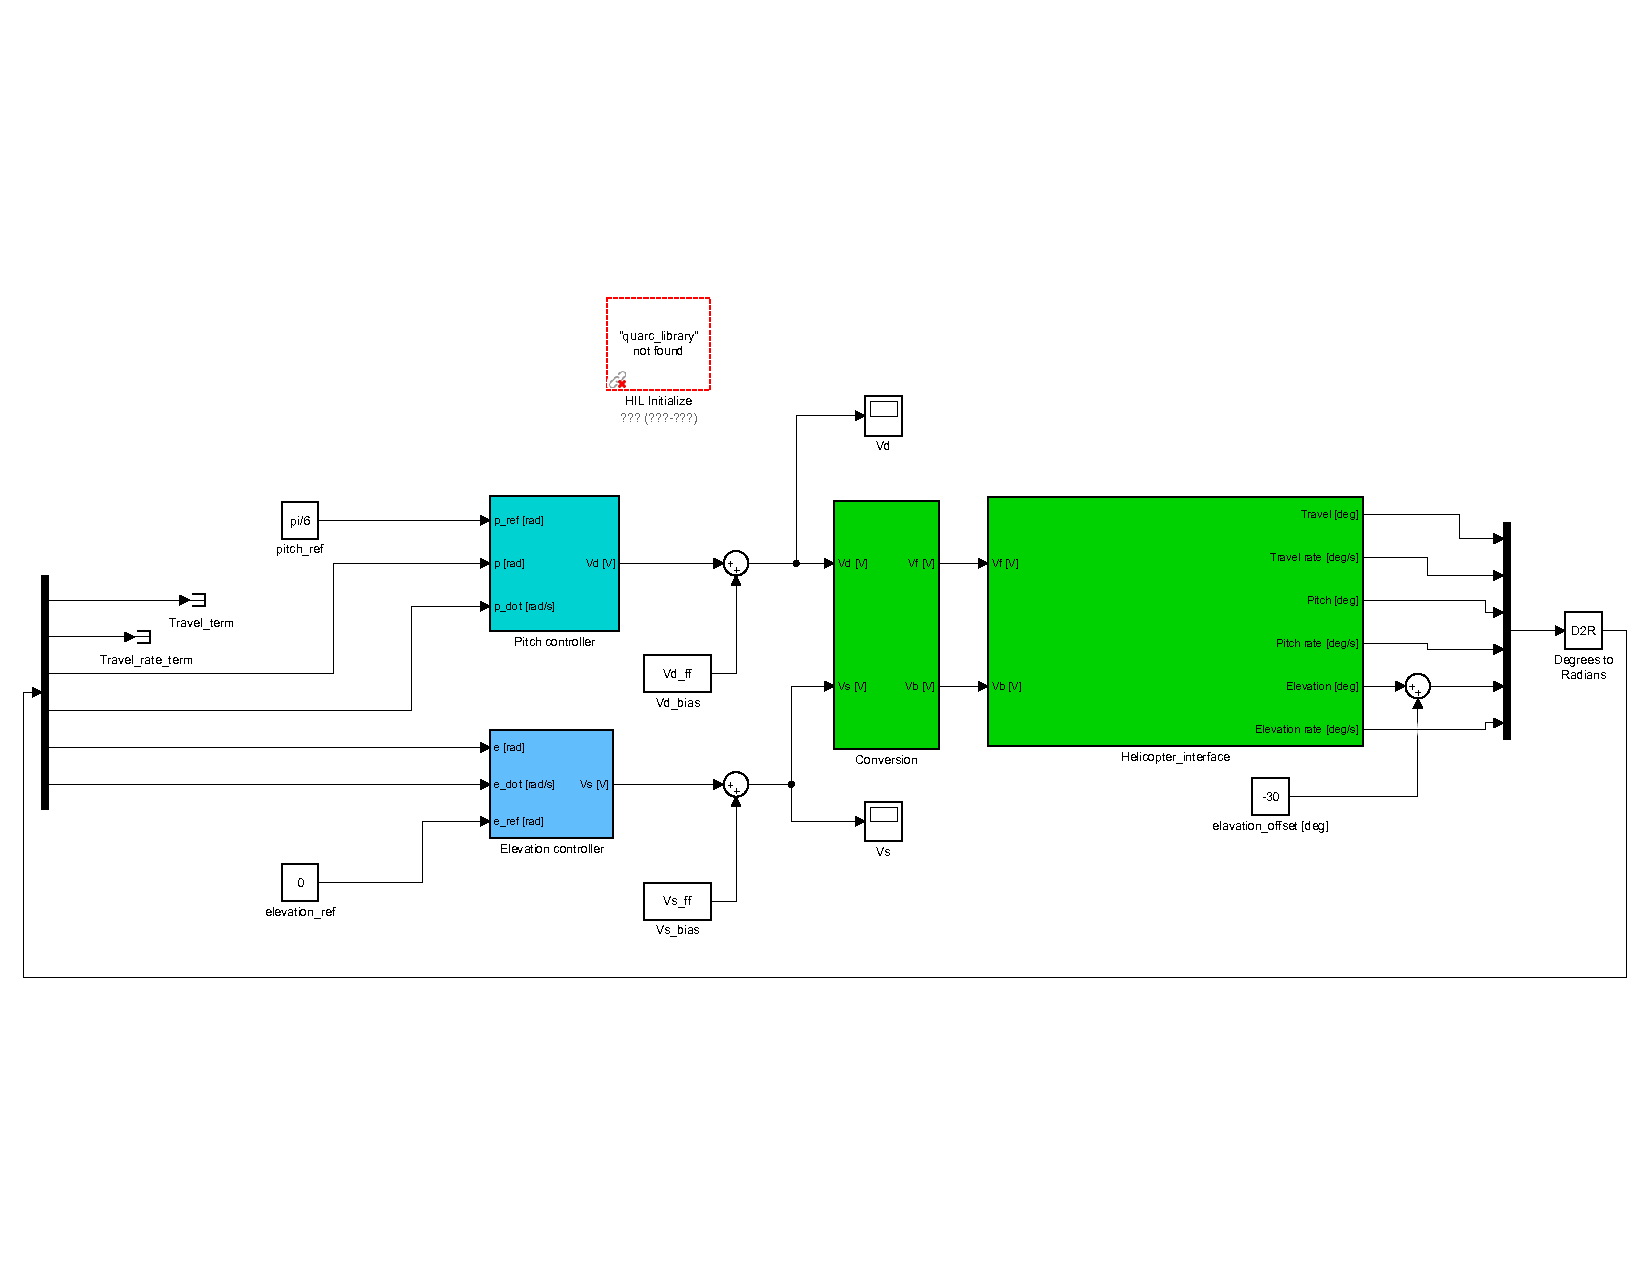
\includegraphics[trim=10 100 10 100, clip, width=\textwidth]{figures/simulink/ex1.pdf}
	\caption{Handed out Simulink model of helicopter with PD pitch controller and PID elevation controller}
\label{fig:sim_start}
\end{figure}

\begin{figure}[!htb]
	\centering
	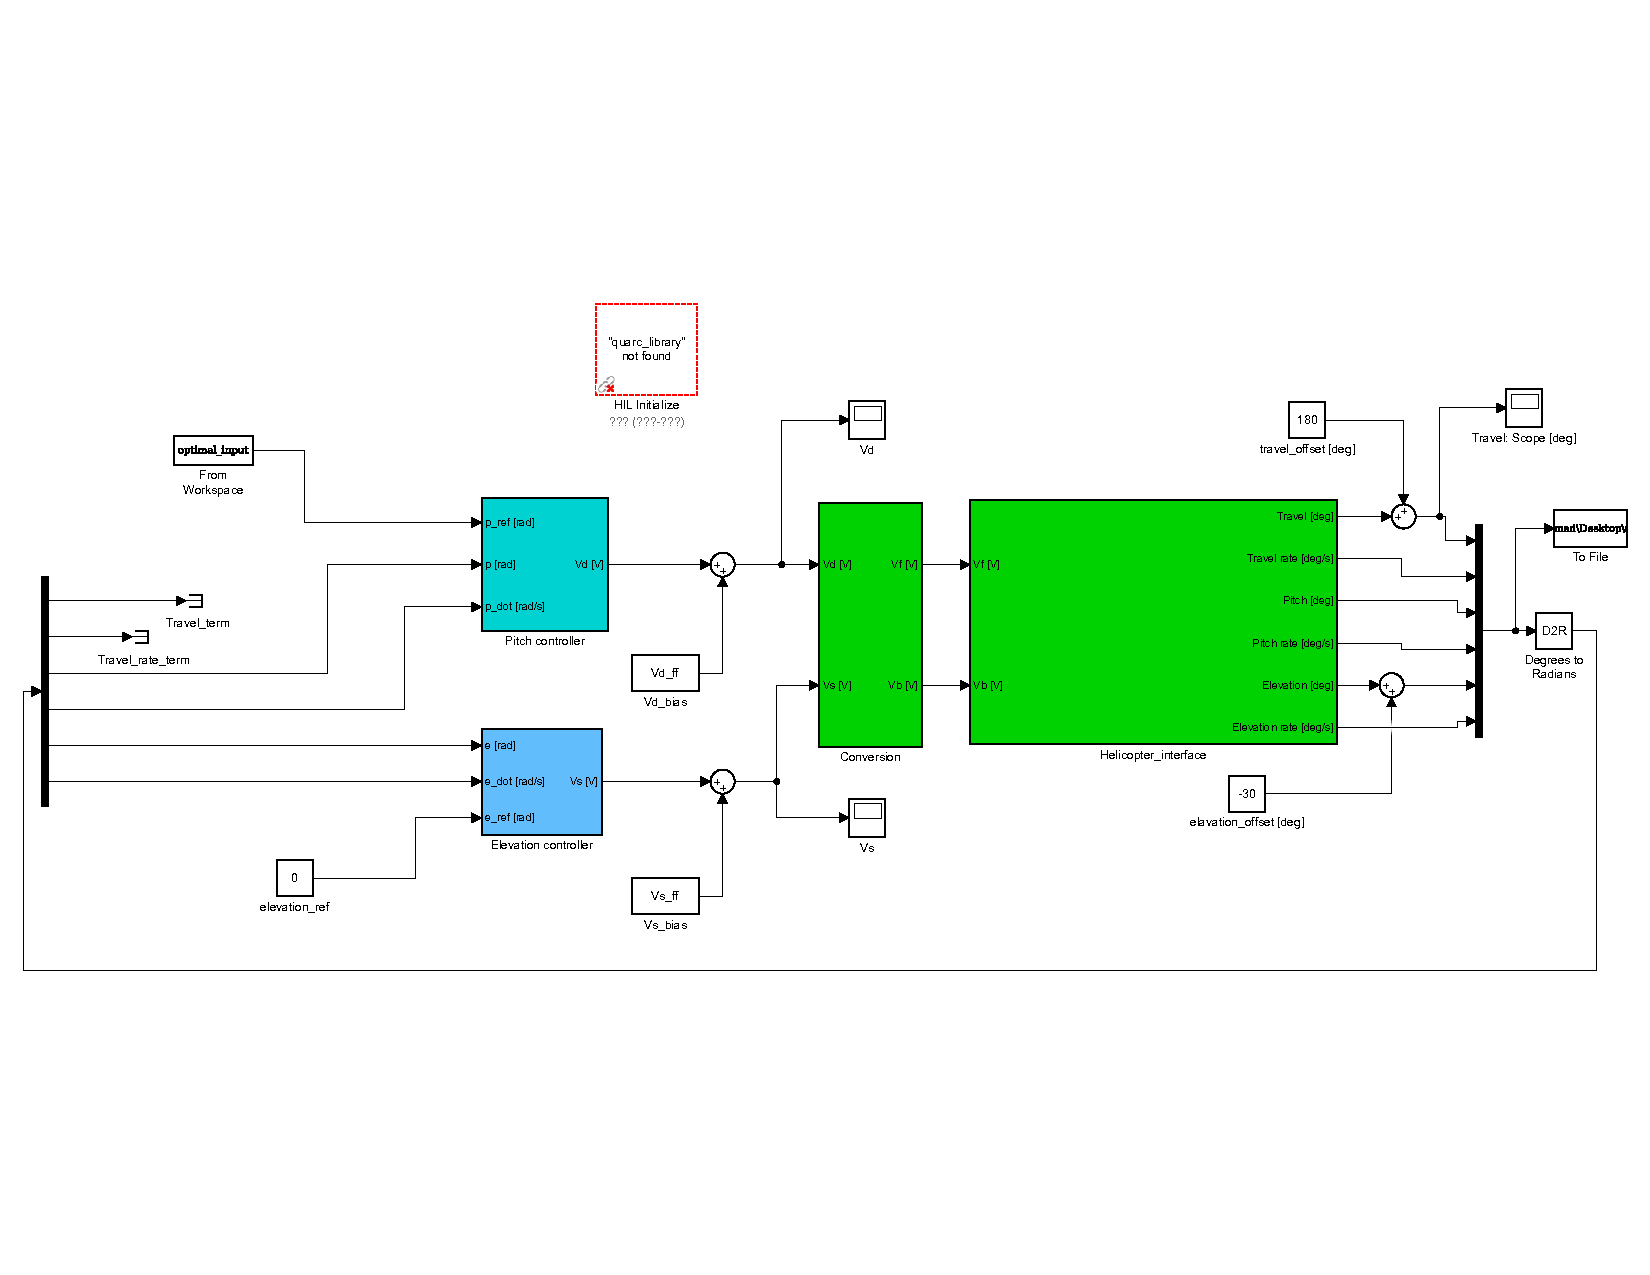
\includegraphics[trim=10 100 10 100, clip, width=\textwidth]{figures/simulink/ex2.pdf}
	\caption{Simulink model with optimization layer on top of basic control layer, no feedback to optimization layer.}
\label{fig:sim_ex2}
\end{figure}


\begin{figure}[!htb]
	\centering
	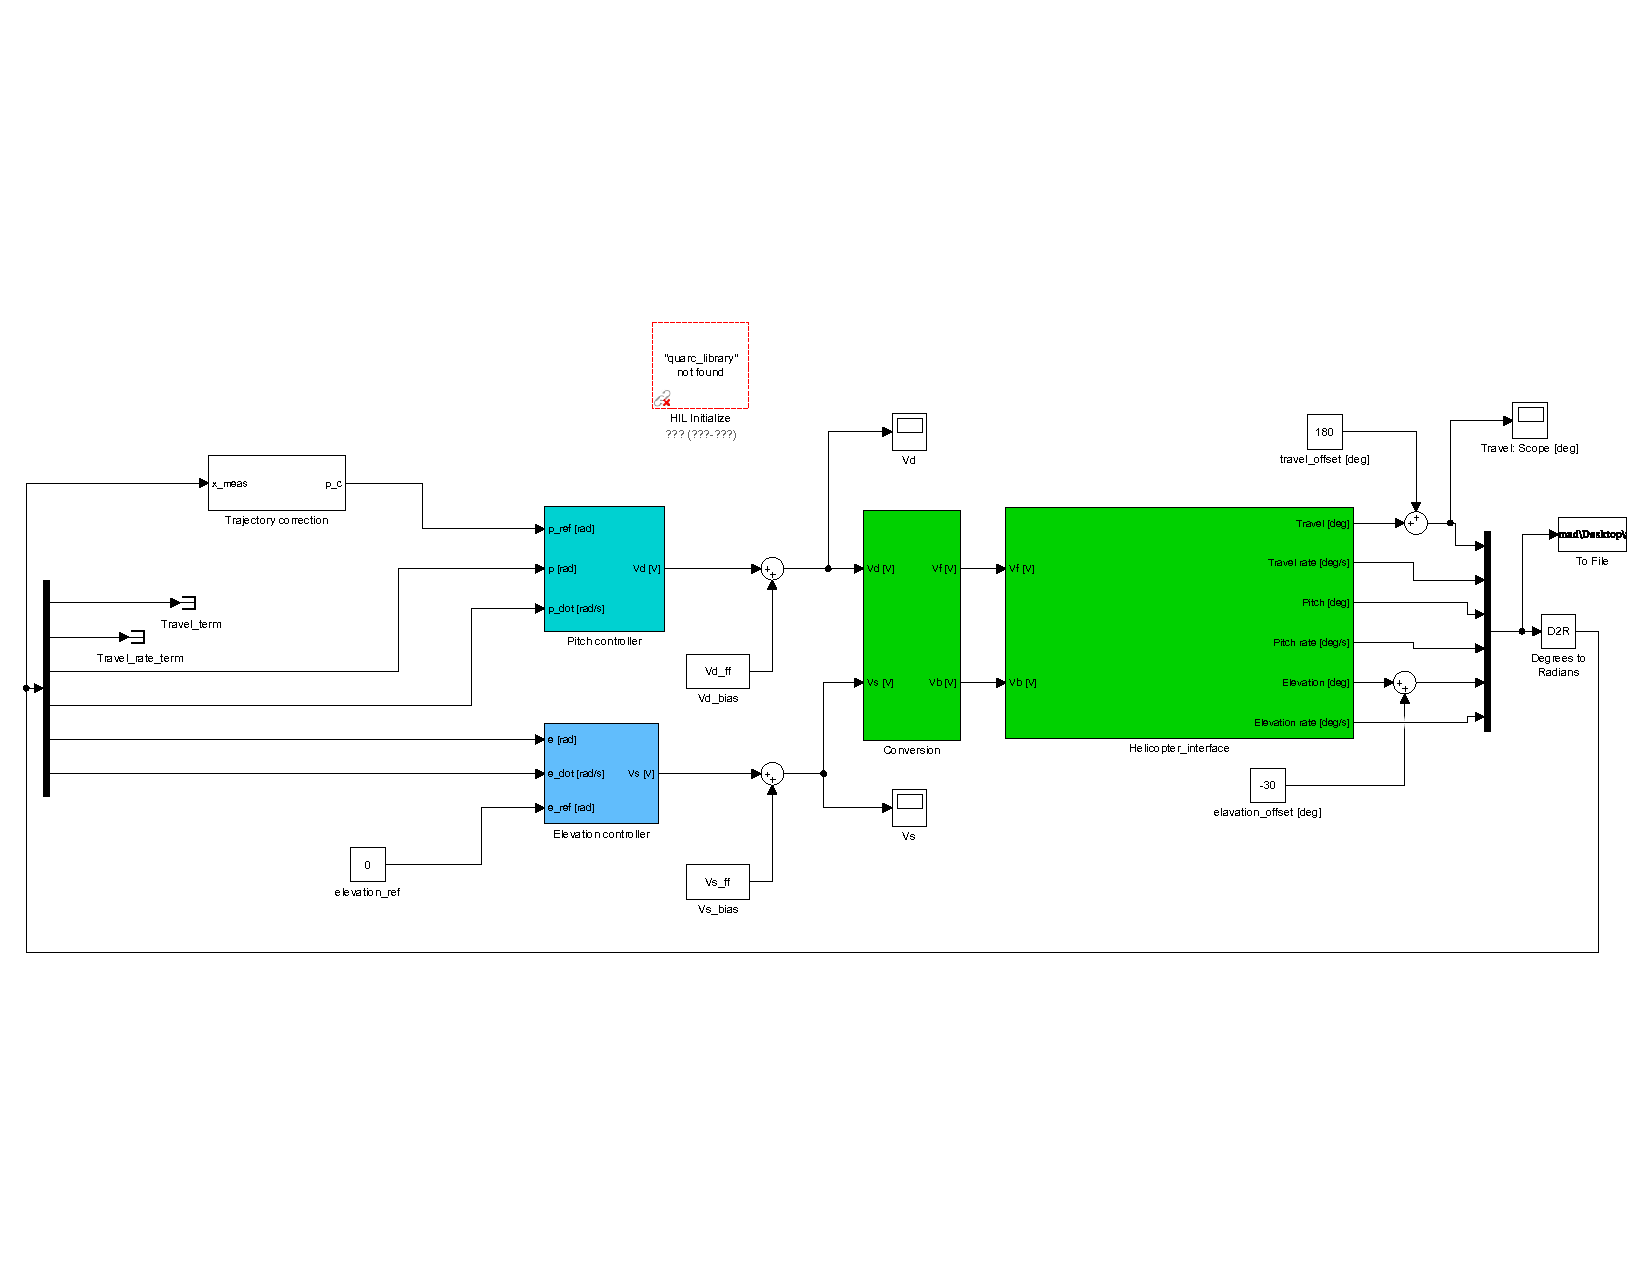
\includegraphics[trim=10 100 10 100, clip, width=\textwidth]{figures/simulink/ex3.pdf}
	\caption{Simulink model with optimization layer on top of basic control layer, this time with feedback to optimization layer in the form of a LQ controller.}
\label{fig:sim_ex3}
\end{figure}

\begin{figure}[!htb]
	\centering
	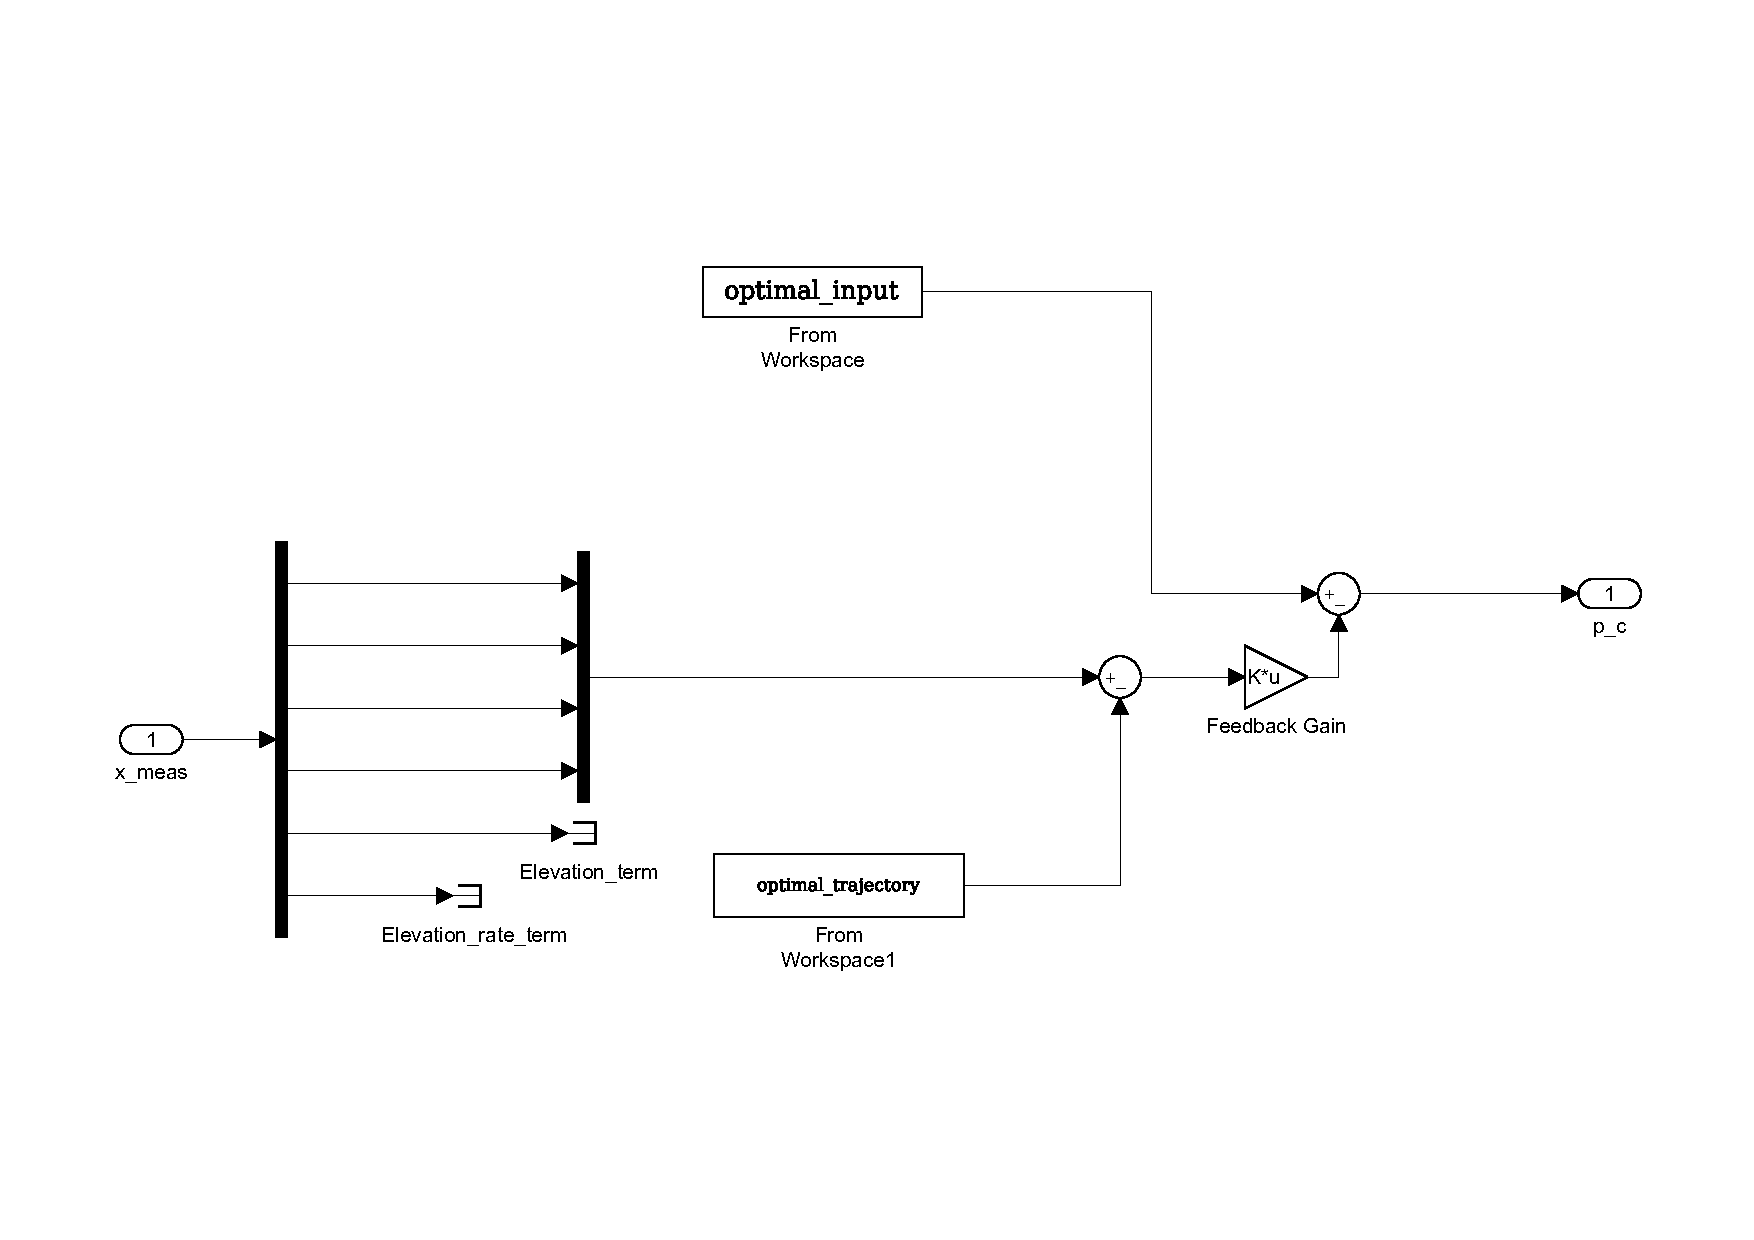
\includegraphics[trim=10 100 10 100, clip, width=\textwidth]{figures/simulink/ex3_feedback.pdf}
	\caption{Detailed view of the LQ controller responsible for feedback.}
\label{fig:sim_ex3_fb}
\end{figure}

\begin{figure}[!htb]
	\centering
	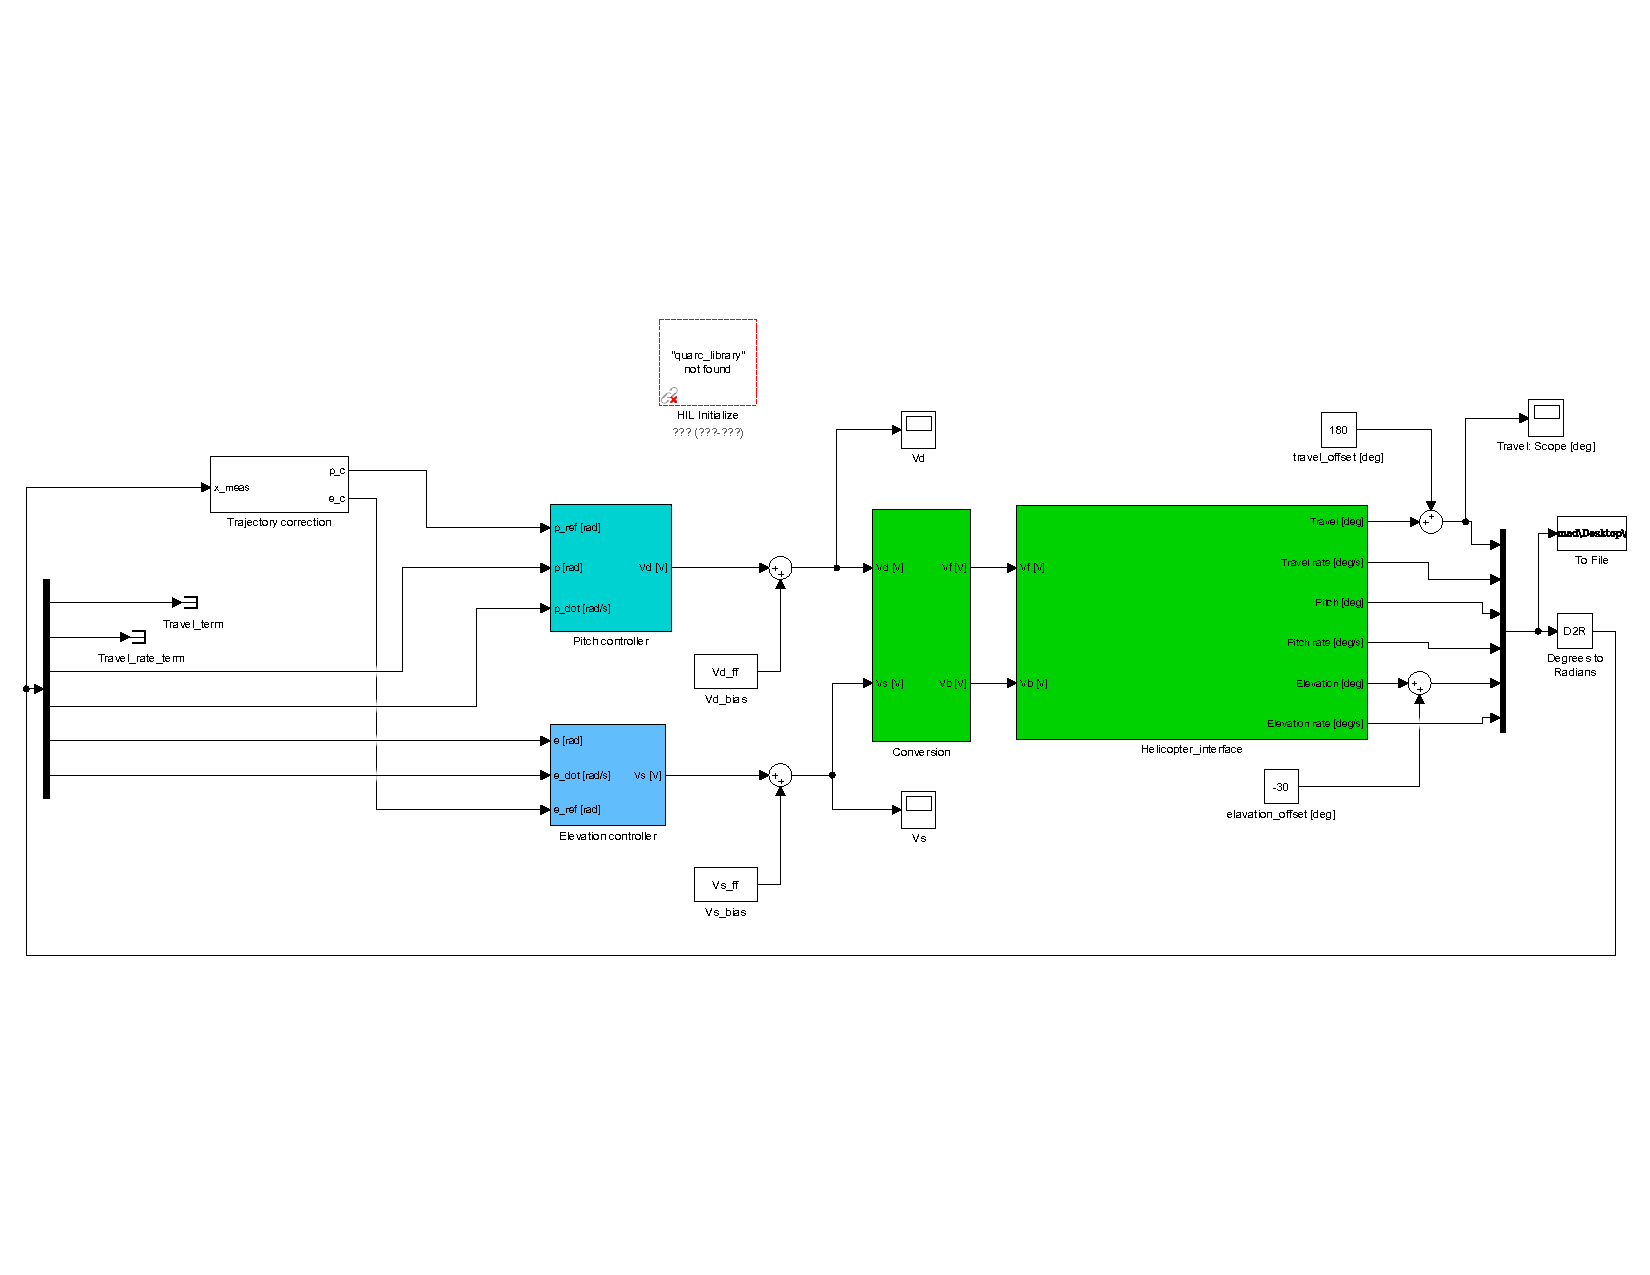
\includegraphics[trim=10 100 10 100, clip, width=\textwidth]{figures/simulink/ex4.pdf}
	\caption{Simulink model with optimization layer on top of basic control layer, this time with feedback to optimization layer in the form of a LQ controller and optimization layer extended to include elevation.}
\label{fig:sim_ex4}
\end{figure}

\begin{figure}[!htb]
	\centering
	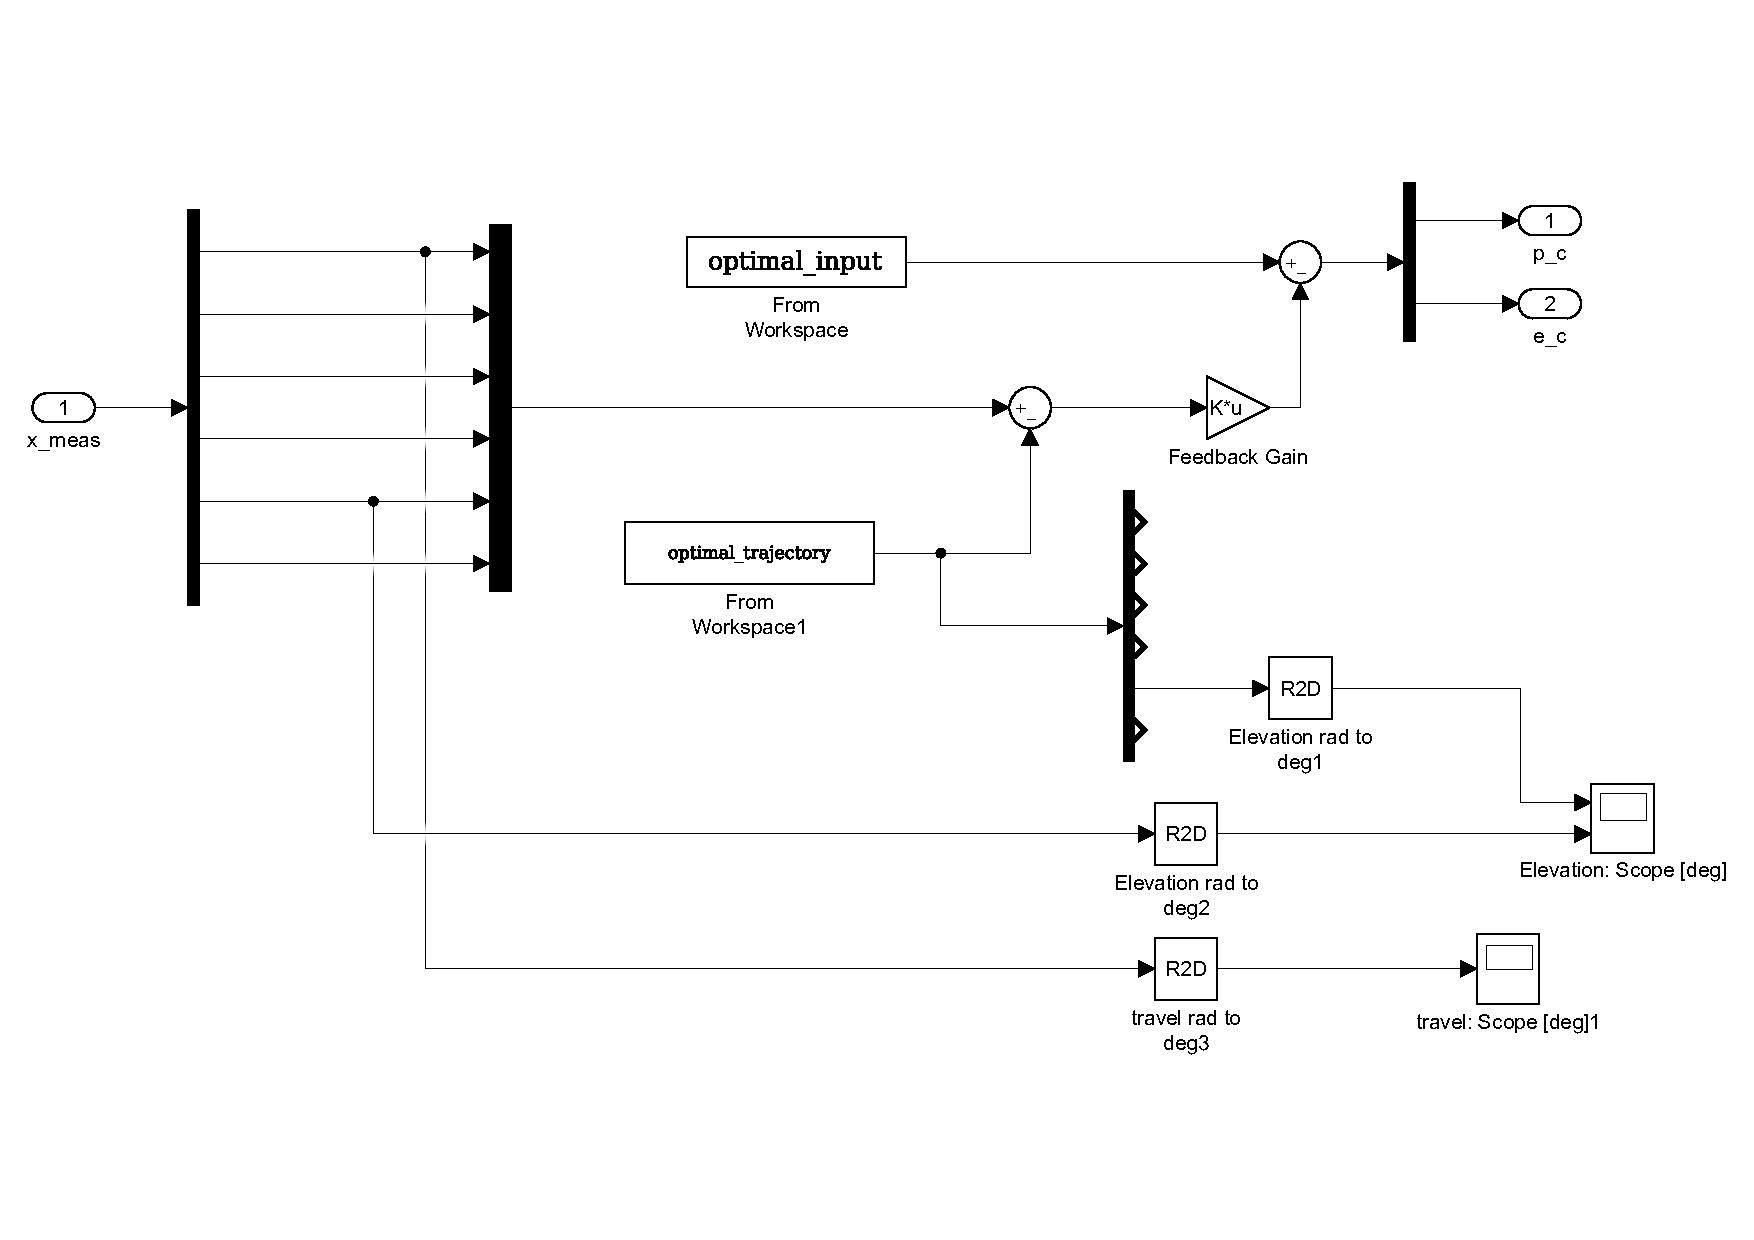
\includegraphics[trim=10 100 10 60, clip, width=\textwidth]{figures/simulink/ex4_feedback.pdf}
	\caption{Detailed view of the extended LQ controller responsible for feedback.}
\label{fig:sim_ex4_fb}
\end{figure}




